%==============================================
\subsection{W–Clearance Connectivity Graph (WCCG)}
\label{subsec:wccg}
\begin{figure*}
  \centering
  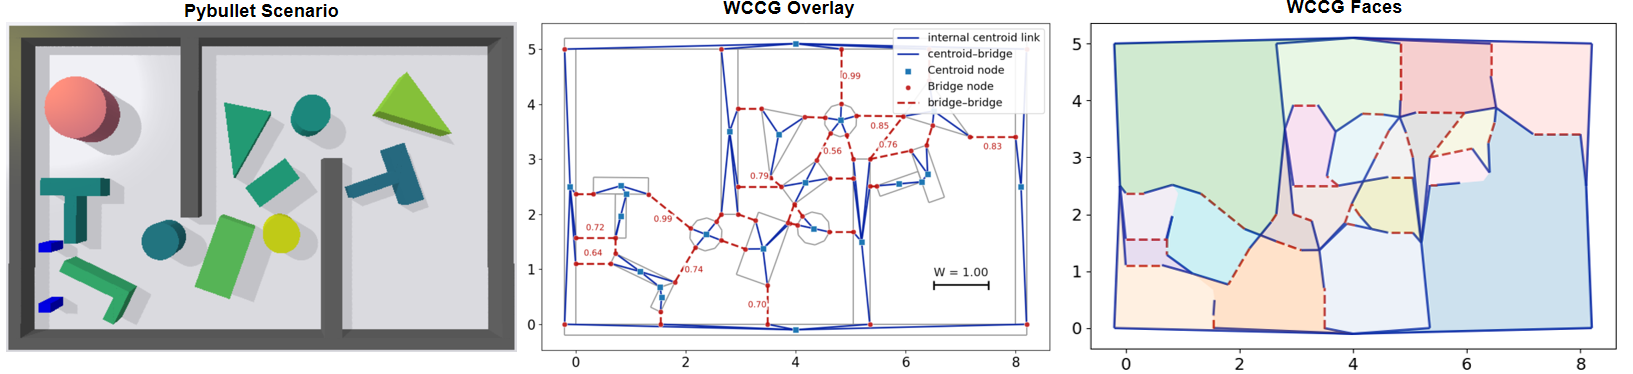
\includegraphics[width=\linewidth]{figures/wccg.pdf}
  \vspace{-4mm}
  \caption{(a) Top–down PyBullet scene (walls/obstacles in gray). 
  (b) w–Clearance Connectivity Graph (w–CCG): blue solid edges are centroid links; red dashed edges are bridge–bridge links annotated with gap widths; blue squares and red circles denote centroid and bridge nodes, respectively; a scale bar shows $W$ (here $W{=}1.00$).
  (c) Faces extracted from the w–CCG, displayed as semi-transparent regions.}
  \label{fig:wccg}
  \vspace{-2mm}
\end{figure*}

To reason about the existence of a traversable path of minimum width~$W$, we
construct a \emph{w–Clearance Connectivity Graph} (WCCG). The graph encodes
obstacle–to–obstacle adjacency under a width threshold: edges appear where the
clearance between obstacles is below~$W$, and nodes summarize convex parts of
obstacles and the bridge points that lie on their boundaries. This discrete
representation allows efficient queries about whether a start
$\mathbf{s}^{\texttt{S}}$ and a goal $\mathbf{s}^{\texttt{G}}$ can be
connected without crossing any gap narrower than~$W$.

%==============================
\subsubsection{Free-Space View and Clearance Requirement}
\label{subsubsec:wccg-decomposition}
Let $\boldsymbol{\Omega}(t)=\{\Omega_1(t),\ldots,\Omega_M(t)\}$ denote movable
obstacles at time $t$, $\mathcal{O}^{\texttt{fix}}$ the static ones, and
$\mathcal{W}$ the workspace. The instantaneous free space is
\begin{equation}\label{eq:free-space}
  \widehat{\mathcal{W}}(t)
  \triangleq \mathcal{W}\setminus\!\big(\mathcal{O}^{\texttt{fix}}\cup\{\Omega_m(t)\}_{m\in\mathcal{M}}\big).
\end{equation}
A path is $W$–feasible iff it maintains clearance at least $W/2$ from the
boundary of $\widehat{\mathcal{W}}(t)$. Conceptually, this equals navigating
in the eroded set
\begin{equation}\label{eq:clearance-space}
  \widehat{\mathcal{W}}^{W}(t)
  \triangleq \{p\in\widehat{\mathcal{W}}(t)\mid \mathrm{dist}(p,\partial\widehat{\mathcal{W}}(t))\ge W/2\}.
\end{equation}
In practice, we \emph{do not} compute~\eqref{eq:clearance-space} explicitly;
instead, we build a discrete graph that is equivalent for connectivity queries.

%==============================
\subsubsection{Graph Construction from Polygonal Obstacles}
\label{subsubsec:wccg-construction}
Given polygonal obstacles decomposed into convex parts, the WCCG
$\mathcal{G}^{W}=(\mathcal{V}^{W},\mathcal{E}^{W})$ is built as follows
(see Alg.\;imp. in \texttt{WClearanceGraph}):

\textbf{(i) Centroid nodes.} For each convex subpolygon we add a centroid
  node; for composite obstacles we also connect adjacent subpolygons by a
  centroid–midpoint–centroid chain.

\textbf{(ii) Bridge nodes.} For each pair of obstacles we compute all
  closest-point pairs $(p_i,p_j)$ between their convex parts whose Euclidean
  distance $d(p_i,p_j)$ is strictly less than $W$ and whose segment is visible
  (no intersection with other obstacles). Each $p_i$ (resp.\ $p_j$) becomes a
  bridge node attached to its subpolygon’s centroid.

\textbf{(iii) Bridge–bridge edges.} Every visible pair $(p_i,p_j)$ with
  $d(p_i,p_j)<W$ yields a bridge–bridge edge whose attribute stores the gap
  width. Centroid–bridge edges form the remainder of $\mathcal{E}^{W}$.

Intuitively, red dashed edges in Fig.~\ref{fig:wccg}(b) mark \emph{narrow
gaps} ($<W$), while blue solid edges organize the interior connectivity of
obstacles.
\subsubsection{Connectivity Test via BugPlanner}
\label{subsubsec:bugplanner-connectivity}
Given start $\mathbf{s}^{\texttt{S}}$ and goal $\mathbf{s}^{\texttt{G}}$, 
we test $W$-width connectivity on the WCCG using a ray-shoot–and–loop-follow procedure 
(Alg.\,\ref{alg:bugplanner}). From a current point, the planner casts a ray toward the goal, 
takes the nearest intersected edge, and then walks the \emph{frontier loop} 
by following the angular order at each vertex. 
If the loop has odd intersection parity with segment $\mathbf{s}^{\texttt{S}}\mathbf{s}^{\texttt{G}}$, 
it is a blocking frontier; 
otherwise an \emph{exit} on the loop (chosen by outward normal toward the goal) 
is taken and the process \emph{re-shoots} from that exit with a tiny bias to avoid degeneracy. 
The algorithm halts either with a straight, collision-free shot to $\mathbf{s}^{\texttt{G}}$ or with a certified blocking loop.

\noindent\textbf{Outputs (topological witness).}
If connectivity holds, the planner returns a frontier–guided \emph{skeleton} $\Sigma$ (an ordered sequence of WCCG edges: center–bridge–center–$\cdots$) that lives on obstacle/frontier adjacency, not necessarily inside the geometric $W$–clear tube. Otherwise, it returns (i) a closed frontier ring and (ii) the set of narrow gap edges on that ring (the \emph{critical gaps}), i.e., edges with width $<W$ that lie on every route between the endpoints and are therefore the minimal widening targets.

\noindent\textbf{From skeleton to a $W$–clear path.}
Under convex decomposition and the angular-order rule, each center–bridge–center segment of $\Sigma$ can be slid continuously onto the boundary of the $W/2$–inflated obstacles, forming a boundary-following curve with cross-gap hops. A small inward normal offset of this curve lies entirely in the $W$–clear free space $\mathcal F_W$. With cleared endpoint disks $\mathbb{B}_{W/2}(\mathbf{s}^{\texttt{S}})$ and $\mathbb{B}_{W/2}(\mathbf{s}^{\texttt{G}})$, short connectors attach the endpoints, yielding a geometric path of clearance at least $W$.

\noindent\textbf{Key implementation details.}
(i) Segment–segment intersections are computed in a vectorized fashion over all candidate edges (AABB culling $+$ linear solve) to obtain the closest hit in one pass.
(ii) Loop following uses the precomputed angular ordering of neighbors at each vertex; the side sign is tracked to stay on the same frontier.
(iii) The re-shoot step adds a tiny directional bias to bypass $s\!\approx\!0$ degeneracy.
(iv) Visualization is incremental: rays, frontier segments, loop edges, and entry/exit points are upda

\begin{theorem}[Complete criterion for a $W$-clear path]
\label{thm:complete-W-test}
Let $\mathcal{O}\oplus \mathbb{B}_{W/2}$ be the Minkowski sum of all obstacles with a radius-$W/2$ disk, and let
$\mathcal{F}_W := \mathbb{R}^2 \setminus (\mathcal{O}\oplus \mathbb{B}_{W/2})$
be the $W$-clear free space.
There exists a collision-free path of clearance at least $W$ from
$\mathbf{s}^{\texttt{S}}$ to $\mathbf{s}^{\texttt{G}}$ \emph{iff}
\begin{enumerate}\itemsep2pt
\item[\textup{(i)}] $\mathbf{s}^{\texttt{S}}$ and $\mathbf{s}^{\texttt{G}}$ lie in the same face (path-connected component) of the W-CCG induced by $\mathcal{F}_W$, and
\item[\textup{(ii)}] the endpoint disks are clear:
$\mathbb{B}_{W/2}(\mathbf{s}^{\texttt{S}})\subset \mathcal{F}_W$ and
$\mathbb{B}_{W/2}(\mathbf{s}^{\texttt{G}})\subset \mathcal{F}_W$.
\end{enumerate}
\end{theorem}

\begin{proof}[Intuitive proof (sketch)]
Convex–decompose all obstacles and inflate each convex piece by a radius $W/2$; assume the endpoint disks $\mathbb{B}_{W/2}(S)$ and $\mathbb{B}_{W/2}(G)$ are free.
\textbf{(i) Discrete skeleton from BugPlanner:}
Running BugPlanner on the $W$–CCG produces a “center $\to$ bridge $\to$ center $\to \cdots$” sequence connecting $S$ to $G$ within one face of the graph.
\textbf{(ii) Slide to the inflated boundary:}
By convexity and the angular-order rule, each center–bridge–center segment can be continuously slid onto the boundary of the inflated obstacles, yielding a boundary-following curve with occasional cross-gap transitions between adjacent inflated pieces.
\textbf{(iii) No premature boundary hits:}
If this slide were to encounter a third inflated piece first, that piece would have offered a nearer bridge in the same angular sector; this contradicts BugPlanner’s neighbor selection by angular order. Hence the slide stays on the intended boundary and designated bridges.
\textbf{(iv) Offset into free space:}
A small inward normal offset of the boundary-following curve lies entirely in the $W$–clear free space $\mathcal{F}_W=\mathbb{R}^2\!\setminus(\mathcal{O}\oplus\mathbb{B}_{W/2})$.
\textbf{(v) Attach endpoints:}
Short connectors through the cleared endpoint disks link $S$ and $G$ to the offset curve, preserving the $W/2$ margin everywhere.
\textbf{(vi) Conclusion:}
The resulting route maintains distance at least $W/2$ to every obstacle, hence a $W$–clear path exists.
\end{proof}



\begin{remark}[Practical check and engineering add-on]
In practice, the test reduces to two steps:
(i) run the W-CCG connectivity between $\mathbf{s}^{\texttt{S}}$ and $\mathbf{s}^{\texttt{G}}$;
(ii) confirm both endpoint disks $\mathbb{B}_{W/2}$ are obstacle-free.
If (i) passes but (ii) fails, we optionally issue a few \emph{away-from-endpoint} pushes to clear the disks; this is an implementation convenience rather than a core part of the method.
\end{remark}

\begin{algorithm}[t]
\small
\caption{BugPlanner for $W$-width connectivity (skeleton witness)}
\label{alg:bugplanner}
\DontPrintSemicolon
\SetKwInOut{Input}{In}\SetKwInOut{Output}{Out}
\Input{$\mathbf{s}^{\texttt{S}}$, $\mathbf{s}^{\texttt{G}}$, WCCG}
\Output{if connected: skeleton $\Sigma$; else: frontier loop $\mathcal{L}$}
$P\leftarrow\mathbf{s}^{\texttt{S}}$,\; $\Sigma\leftarrow[\ ]$\;
\While{true}{
  \If{segment $P\mathbf{s}^{\texttt{G}}$ hits no edge}{\Return $\Sigma \cup \{\texttt{straight}(P,\mathbf{s}^{\texttt{G}})\}$}
  Build loop $\mathcal{L}$ by angle-follow from the hit edge; append traversed edges to $\Sigma$\;
  \If{$\mathrm{parity}(\mathcal{L},\,\mathbf{s}^{\texttt{S}}\mathbf{s}^{\texttt{G}})$ is odd}{\Return $(\emptyset,\mathcal{L})$}
  Choose exit $e$ on $\mathcal{L}$ (outward normal $\to\,\mathbf{s}^{\texttt{G}}$); append arc to $\Sigma$; $P\leftarrow e$ (tiny bias)\;
}
\end{algorithm}

\begin{remark}[Skeleton $\to$ path]
BugPlanner certifies connectivity via a frontier skeleton. A geometric $W$–clear path is obtained by sliding $\Sigma$ onto the $W/2$–inflated boundary, offsetting slightly inward into $\mathcal F_W$, and attaching the cleared endpoint disks. This mapping is continuous and preserves homotopy.
\end{remark}